\chapter{Experiments}

Several experiment setups were designed to focus on the effect of temperature on the mote hardware and link quality and executed in two locations: a temperature-controlled server room in the basement and a large empty storage space.
We chose these locations for their low visitation frequency, since the presence of moving objects, especially humans, alters the link quality, which of course was undesirable.

In the server room, a space of about $3x12$m was available, with a thick load-bearing concrete wall on the one side and metallic server racks on the other.
This environment quickly proved too reflective for the transmissions, meaning that signal power was ``trapped'' between these two obstacles, which made for a very good link quality, which was the opposite of what we needed.
We tried a power setting of 3 (-25dBm), but even at the maximum distance the link was without bit errors, therefore we settled on power setting 2 (below -25dBm), which required the motes to be very close to each other at about 30cm.
Due to the difficulty of manipulating link quality with fine granularity, we only ran one experiment in this room and then relocated the setup.

The storage room was larger at about $10x15$m with a window front and many shelves on the walls.
Here we could use power setting 3 at about 3m distance and very accurately manipulate link quality.
Therefore we used this location for the remaining experiments.
All experiments were done using the on-board PCB antenna, sending on channel 26 to minimize WiFi interference.


\section{Clock Drift}

The Tmote Sky uses a MSP430 microcontroller clocked an integrated ring oscillator called the \ac{DCO}.
Since the generated clock frequency varies with temperature, voltage and from chip-to-chip, the \ac{DCO} can be fine-tuned using a modulation functionality.
During booting, TinyOS calibrates the \ac{DCO} using the external low-current 32.756Hz watch crystal to generate a more accurate 1MHz clock.
It should be noted, that calibration only occurs after a reset, and not periodically during program execution.

We noticed a problem, where serial communication stopped working after heating the nodes above $55-60\,^{\circ}\mathrm{C}$. Below this temperature the problem could be mitigated by resetting the mote to trigger a recalibration of the \ac{DCO}.
We therefore looked at the output of the \ac{UART} module with a logic analyzer and measured the how the selected baudrate changes over temperature.
Since the baudrate is generated by scaling the \ac{DCO}, relative baudrate error is equivalent to relative \ac{DCO} error.
Figure~\ref{fig:baudrate_error} shows the relative error of four baudrates over temperature.
We calculate an average temperature clock drift coefficient of $-0.367\%/\,^{\circ}\mathrm{C}$, which is within the typical range according to the datasheet. Similar coefficients were found by Z{\'u}{\~n}iga~\etal~\cite{Zuniga2013}.

\begin{figure}[t]
	\subfigure[Relative error of four baudrates.] {
    	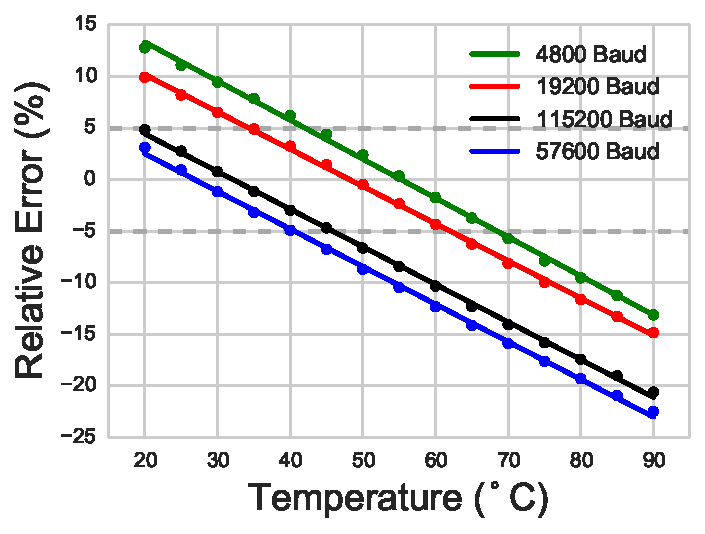
\includegraphics[width=0.5\columnwidth]{figures/baudrate_error}
    	\label{fig:baudrate_error}
    }
    \subfigure[Relative error of \acs{DCO} calibration.] {
	    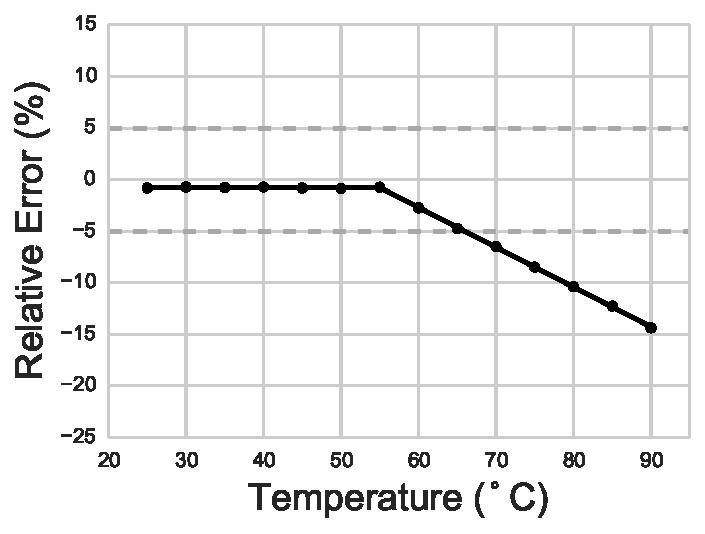
\includegraphics[width=0.5\columnwidth]{figures/reboot_dco_drift}
	    \label{fig:reboot_drift}
	}
	\subfigure[Relative error of corrected baudrate.] {
	    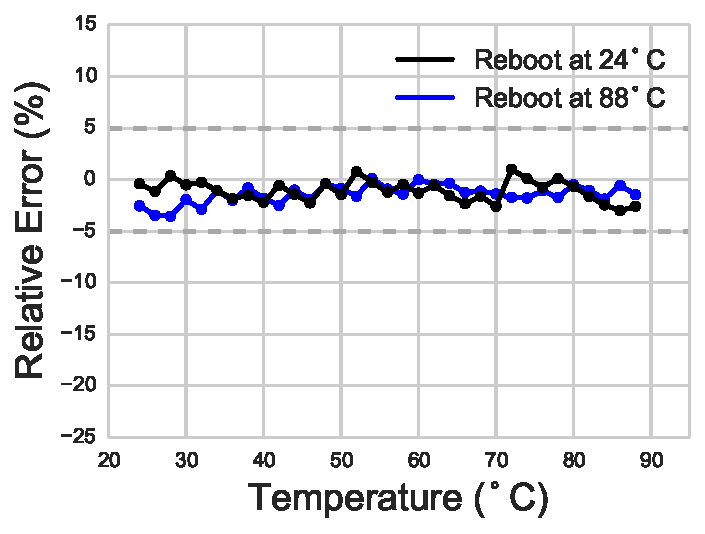
\includegraphics[width=0.5\columnwidth]{figures/baudrate_correction_error}
	    \label{fig:baudrate_look_up_error}
	}
	\subfigure[Values of baudrate correction look-up table.] {
	    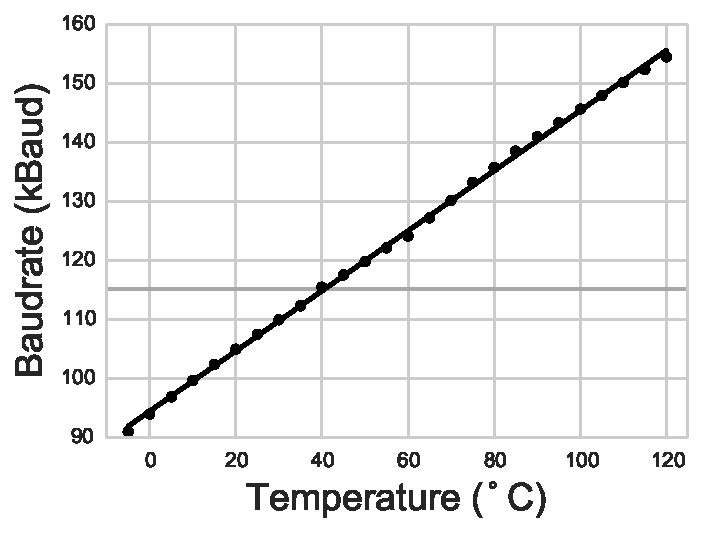
\includegraphics[width=0.5\columnwidth]{figures/baudrate_correction_table}
	    \label{fig:baudrate_look_up}
	}
	\caption{\acs{UART} and \acs{DCO} calibration errors vs. temperature. Note that \acs{UART} can tolerate up to $\pm5\%$ error.}
\end{figure}

We then measured the relative baudrate error after rebooting over temperature.
As shown in Figure~\ref{fig:reboot_drift}, the TinyOS implementation of the \ac{DCO} calibration only works until $55\,^{\circ}\mathrm{C}$, after which it has no corrective effect on CPU frequency, making periodic \ac{DCO} calibration during program execution ineffective.

We chose not to correct clock drift directly, but counteract the effect on baudrate, by creating a lookup-table of ``inverse'' correction baudrates for 115.2kbps and applying it with temperature as shown in Figure~\ref{fig:baudrate_look_up}.
Since calculation of prescaler values at runtime is costly, the look-up table contains precalculated values, which are then copied into the registers at runtime.
The on-board sensor provides temperature to the \ac{UART} module which then selects new prescaler values from the look-up table for every $5\,^{\circ}\mathrm{C}$, which shows as a sawtooth pattern in the resulting relative error of the corrected baudrate as shown in Figure~\ref{fig:baudrate_look_up_error}.

Note that the receiver can still correctly read serial data if the relative error does not deviate more than $\pm5\%$. During reception the falling edge of the startbit is used to synchronize the sampling points of all bits and with 8 databits, 1 startbit and 1 stopbit (8N1 configuration), the stopbit must be sampled during the last $10\%$ of reception time, hence an error tolerance of $\pm5\%$.
For example, the tolerance for 7-bit transfers (9 baudtimes) increases to $\pm5.56\%$.

\todo{last paragraph is a bit cryptic. Overthink it.}

\section{Bit Error Patterns}

We designed two experiments to investigate the results of Schmidt~\etal~\cite{Schmidt2013}, in particular the effect of temperature and hardware revision on bit error distribution.

\subsection{Effects of board layout}
\label{subsec:effects_of_board_layout}

While both versions we used are drop-in replacements for the Telos design devised by Polastre~\etal~\cite{Polastre2005}, the newer MTM-CM5000 version uses a slightly different schematic and different board layout.
Notable differences include the 3V voltage regulator and the layout of the radio circuitry.

In the experiment a pair of CM5000 and original motes transmitted to two CM5000 and two original motes.
This redundant placement shown in Figure~\ref{fig:8_mote_setup} was chosen so that the same transmission was received by both types.
Over the course of six days the four transmitters sent 563.500 messages each, totalling 2.254.000 transmitted messages at power setting 2. Of those transmitted messages a total of 5.280.369 messages were received, 2.497.744 of which had at least one bit error.
The experiment was located in a large climate-controlled server room in the basement, therefore the temperature remained within $20-25\,^{\circ}\mathrm{C}$ with no other changes in the environment.

\begin{figure}[H]
	\centering
	\begin{tikzpicture}
		\newcommand\receiver[5]{%
		    \begin{scope}[xshift=#1cm,yshift=#2cm,rotate=#3]
		        \draw[fill=#4] (0,0) rectangle (1,2.1);
		     	\draw[fill=black!10] (0.33,0.1) rectangle (0.66,-0.45);
		     	\draw[snake=snake, white, segment amplitude=1.75, segment length=5, line width=1.25pt] (0.1, 1.95) -- (0.9, 1.95);
		     	\node at (0.5cm, 1.05cm) {#5};
		    \end{scope}
		}
		\newcommand\transmitter[5]{%
			\receiver{#1}{#2}{#3}{#4}{#5};
		    \begin{scope}[xshift=#1cm,yshift=#2cm,rotate=#3]
		     	\draw[snake=expanding waves, segment angle=40, segment length=7] (0.5,2) -- (0.5,3);
		    \end{scope}
		}

		% new = red, old = blue
		% new transmitter
		\transmitter{3}{7}{-65}{motered}{0};
		\transmitter{3.675}{5.5}{-65}{motered}{1};		

		% new transmitter
		\transmitter{0}{2}{-65}{moteblue}{2};
		\transmitter{0.675}{0.5}{-65}{moteblue}{3};

		\receiver{13}{0}{180}{motered}{7};
		\receiver{13}{3}{180}{moteblue}{6};
		\receiver{13}{6}{180}{motered}{5};
		\receiver{13}{9}{180}{moteblue}{4};

		% labels
		\node at (3, 7.75) {CM5000};
		\node at (0, 2.8) {Original};

		\node at (3, -1.5) {Transmitters};
		\node at (10.5, -1.5) {Receivers};
	\end{tikzpicture}
	\caption{Experiment setup from above with four transmitters and receivers.}
	\label{fig:8_mote_setup}
\end{figure}

Note that the CM5000 motes required to be physically closer to the receivers at the same power setting to have similar link quality as the original motes.
This might be hinting at a difference in range between the two hardware layouts, however, our experiment was not setup to systematically investigate range.

In the initial evaluation we noted some significant differences in the quality of some links, were the co-located transmitters are sending to the same receiver.
For example, the link 3-5 is of very good quality with over 99\% PRR, however link 2-5 shows quite the opposite with less than 1\% PRR, even though both transmitters a located at the same distance and angle from the receiver.
This confirms the findings of Baccour~\etal~\cite{Baccour2012}, specifically that link quality is anisotropic, \ie the communication range exhibits a nonspherical pattern.
More exhibitions of this behavior can be found in the complete table of link qualifiers in the Appendix as Table~\ref{tab:8mote_link_qualities}.

Further analysis revealed the same bit and symbol error patterns as first discovered by Schmidt~\etal~\cite{Schmidt2013}, which state that within any transmitted symbol, the first three MSB are more likely to break than the LSB and that symbols with the MSB set to 1 (\ie 0x8 to 0xF) are more likely to brea.
The probability of bit errors are plotted in Figure~\ref{fig:8mote_bit_errors}, with the first 12 bytes (96 bits) consisting of the message header with partially fixed content and the remaining 80 bytes are the constant payload, made up of two 32 byte patterns of 0x0000, 0x1111, ..., 0xFFFF, and one 16 byte pattern of 0x00, 0x11, ..., 0xFF.

\begin{figure}[H]
	\subfigure[XL symbol influence.] {
    	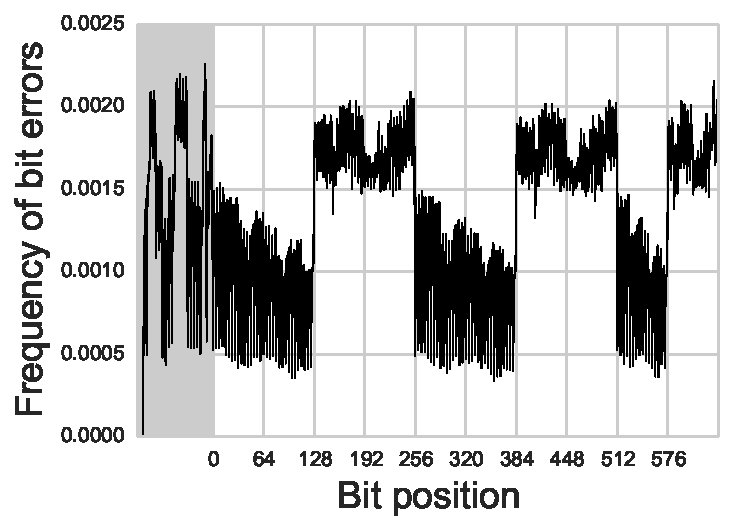
\includegraphics[width=0.5\columnwidth]{figures/8mote_0-5_xor}
    	\label{fig:8mote_bit_errors_xl}
    }
    \subfigure[L symbol influence] {
	    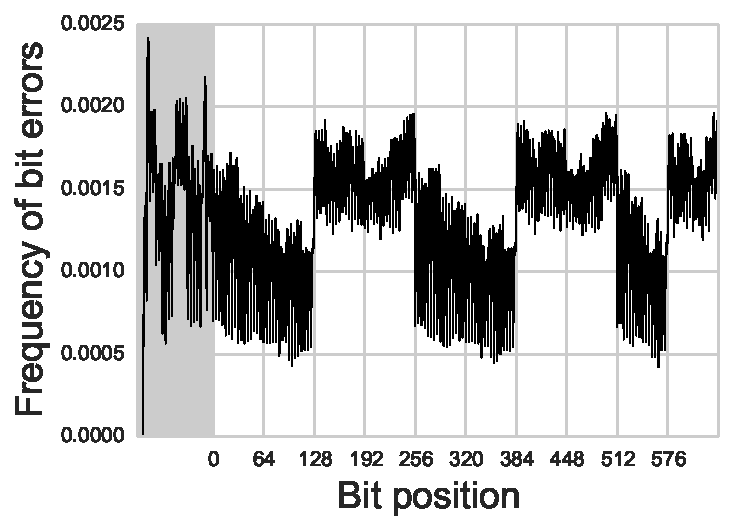
\includegraphics[width=0.5\columnwidth]{figures/8mote_1-6_xor}
	    \label{fig:8mote_bit_errors_l}
	}
	\subfigure[M influence.] {
	    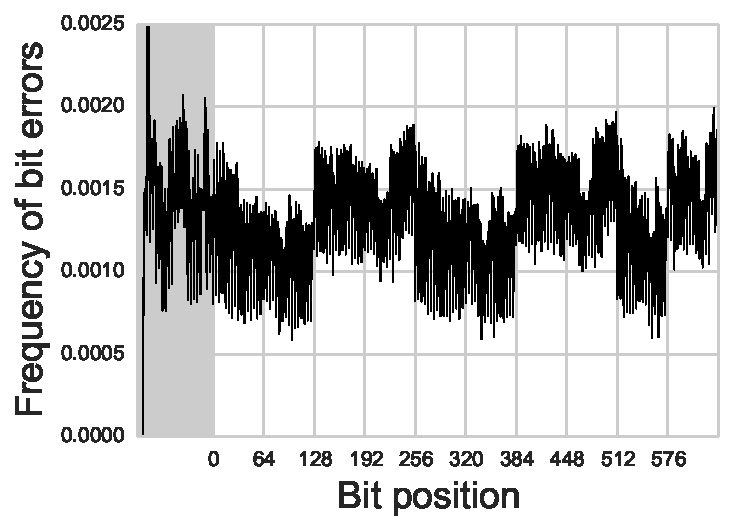
\includegraphics[width=0.5\columnwidth]{figures/8mote_2-6_xor}
	    \label{fig:8mote_bit_errors_m}
	}
	\subfigure[S influence.] {
	    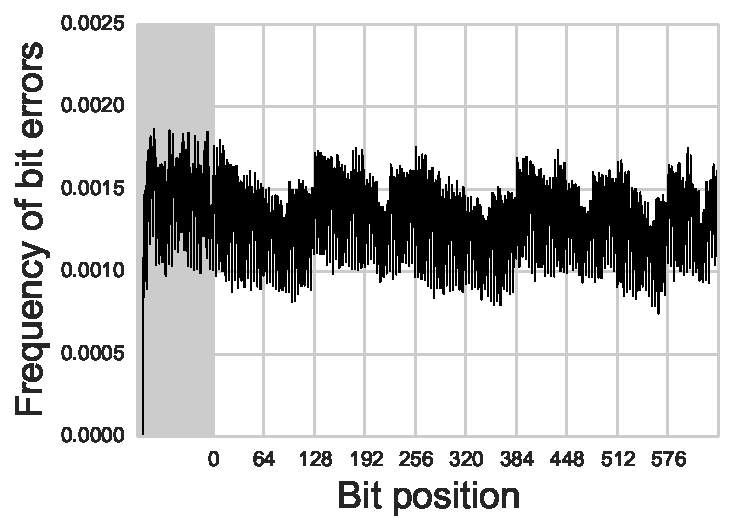
\includegraphics[width=0.5\columnwidth]{figures/8mote_2-7_xor}
	    \label{fig:8mote_bit_errors_s}
	}
	\caption{Four magnitudes of symbol content influence on bit error pattern.}
	\label{fig:8mote_bit_errors}
\end{figure}

We were able to confirm the findings of Schmidt~\etal{} and extend them with a classification of the influence of symbols on bit error probability.
The subfigures show four magnitudes of this phenomenon, ranging from and extreme to almost no difference between symbols, named XL, L, M and S.
The remaining links can be classified into these four categories as done in Table~\ref{tab:8mote_bit_error_link_classification}.

\begin{table}[H]
	\begin{tabularx}{\linewidth}{|c*{4}{|c}|}
	\hline
	\T \cellcolor{slightgray} Receiver	& \multicolumn{1}{X|}{\cellcolor{motered} \centering Sender 0} & \multicolumn{1}{X|}{\cellcolor{motered} \centering Sender 1} & \multicolumn{1}{X|}{\cellcolor{moteblue} \centering Sender 2}	& \multicolumn{1}{X|}{\cellcolor{moteblue} \centering Sender 3}\\
	\hline

	\cellcolor{moteblue}\T 4 & S  & n/a & n/a & n/a \B\\
	\hline
	\cellcolor{motered}\T  5 & XL & XL  & L   & XL  \B\\
	\hline
	\cellcolor{moteblue}\T 6 & XL & L   & M   & n/a \B\\
	\hline
	\cellcolor{motered}\T  7 & L  & n/a & S   & L   \B\\
	\hline 
	\end{tabularx}

	\caption{Classification of all links with enough bit errors (otherwise marked with n/a).}
	\label{tab:8mote_bit_error_link_classification}
\end{table}


\section{Packet Reception Rate}
\label{sec:packet_reception_rate}

The effect of temperature and other environmental factors on link quality has most thoroughly been investigated (\cite{Wennerstrom2013}, \cite{Boano2013}, \cite{Boano2014}, \cite{Zuniga2013}) with the conclusion that all measurements of link quality deteriorate with higher temperature, as one would expect.
However, Boano~\etal{} showed in their experiments that this behavior is not symmetrical, since heating the transmitter caused a more significant drop in \ac{PRR} than heating the receiver~\cite{Boano2013}.

To replicate these results we used the same experiment setup as described in Subsection~\ref{subsec:effects_of_temperature}, but with random payload as message content.
We fixed mote rotation to create a link that is just starting to deteriorate at $50\,^{\circ}\mathrm{C}$, so that at low temperatures the link is of good quality, while at very high temperatures the link will break.

In the experiment we increased the temperature of the mote in box 0 in steps of $5\,^{\circ}\mathrm{C}$ and $10\,^{\circ}\mathrm{C}$ up to $80\,^{\circ}\mathrm{C}$ and kept the mote on box 1 at constant $30\,^{\circ}\mathrm{C}$, while sending 180.000 messages back and forth.
Then we repeated this, but heated box 1 and kept box 0 temperature constant.
To cancel out environmental factors we ran this experiment four times over two days, so we could then pick the two results with the least interference.

For the evaluation we plotted the normalized \ac{PRR} of messages sent one mote and received by the other mote over temperature and time and included \ac{BER} and \ac{LQI} and \ac{RSSI} values to illustrate link quality.
Figure~\ref{fig:prr_link_01} shows messages sent from mote 0 addressed to mote 1 for both temperature cycles, while Figure~\ref{fig:prr_link_10} shows the opposite direction.
It becomes immediately clear that higher temperature of either transmitter or receiver makes the link worse, however, this behavior is neither linear nor symmetrical.

\subsection{Effects of temperature on \acs{PRR} and \acs{BER}}

In Figure~\ref{fig:prr_link_01} the decrease in \ac{PRR} is small and relatively symmetrical up to about $65\,^{\circ}\mathrm{C}$, however, past that point we see a dramatic change, with the increments in temperature translating very strongly into significant drops in \ac{PRR}.
The drop in \ac{PRR} is not symmetrical and becomes much more pronounced, when the receiver is heated than when the transmitter is heated, especially visible in the last increment from $70\,^{\circ}\mathrm{C}$ to $80\,^{\circ}\mathrm{C}$.

This asymmetry is even more extreme in link 1-0, shown in Figure~\ref{fig:prr_link_10}, where heating the receiver beyond $70\,^{\circ}\mathrm{C}$ will cause an almost complete loss of message reception.
Interesting is the little dip in \ac{PRR} around $50\,^{\circ}\mathrm{C}$ in Subfigure~\ref{fig:prr_link_10_receiver}, which was present in this link in all four experiments with varying intensity. We suspect that this is a non-linearity in the radio, cases of which have also been reported by Boano~\etal.

The \ac{BER} acts like an inverse function of \ac{PRR}, since higher \ac{BER} yields more messages with at least one bit error.
Noise on \ac{PRR} is visible in the standard deviation of \ac{BER} as exemplified by Subfigure~\ref{fig:prr_link_10_transmitter}.

\subsection{Effects of temperature on \acs{LQI} and \acs{RSSI}}

The \ac{LQI} is a very good mirror of the \ac{PRR} of messages without error.
When the receiver is kept at a constant temperature, the values decrease almost linearly with temperature of the transmitter.
This is not the case when the receiver is heated, where a linear correlation to temperature does not to exist, but is still very similar to the behavior of \ac{PRR}.
We therefore can confirm, that \ac{LQI} is a good source for an estimate on \ac{PRR}.

This is very much not the case with \ac{RSSI}, which has much lower resolution that \ac{LQI} and exhibits hysteresis and non-linearities~\cite{Boano2013}.
While in Figure~\ref{fig:prr_link_01}, \ac{RSSI} ends up being lower when the receiver is heated than when it is constant, Figure~\ref{fig:prr_link_10} shows very similar values, even though \ac{PRR} is radically different.

It is also noteworthy that contrary to \ac{LQI}, \ac{RSSI} attempts to describe signal strength (\ie the power level being received by the antenna), which of course does not change, when the transmitter is at constant temperature.
Therefore, without temperature information, the \ac{RSSI} value is misleading, since it represents the power level not at the antenna, but at the signal amplifying stage 
Therefore \ac{RSSI} is usable for a very inaccurate estimate of link quality at best, with little to no difference between receiver and transmitter temperature.

\begin{figure}[t]
	\subfigure[Constant receiver, increasing \newline transmitter temperature.] {
		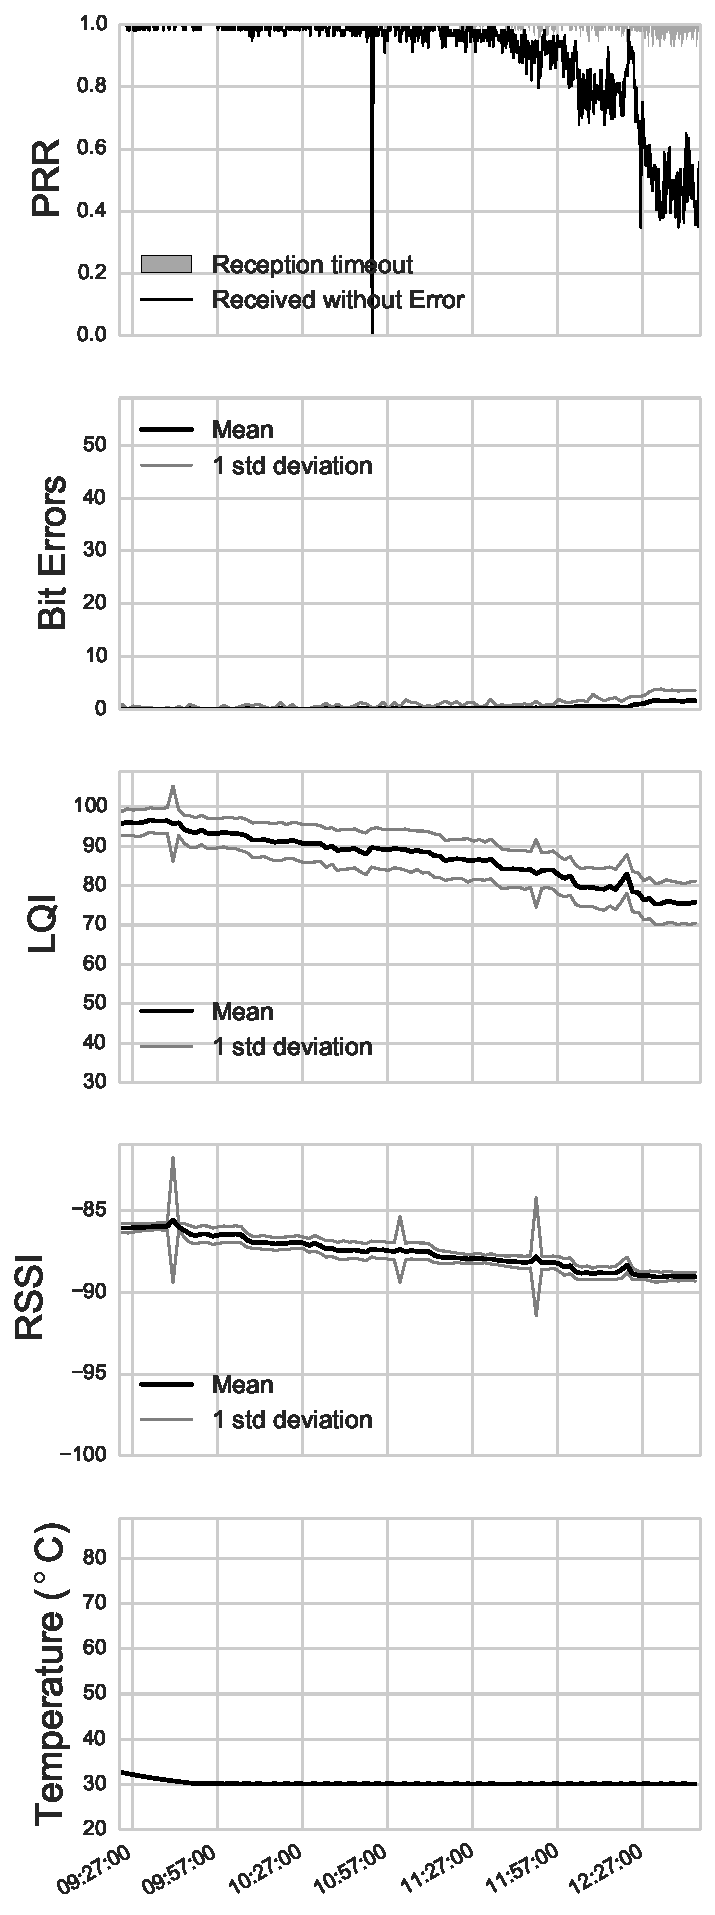
\includegraphics[width=0.475\columnwidth]{figures/prr_0-1_transmitter}
		\label{fig:prr_link_01_transmitter}
	}
	\subfigure[Increasing receiver, constant \newline transmitter temperature.] {
		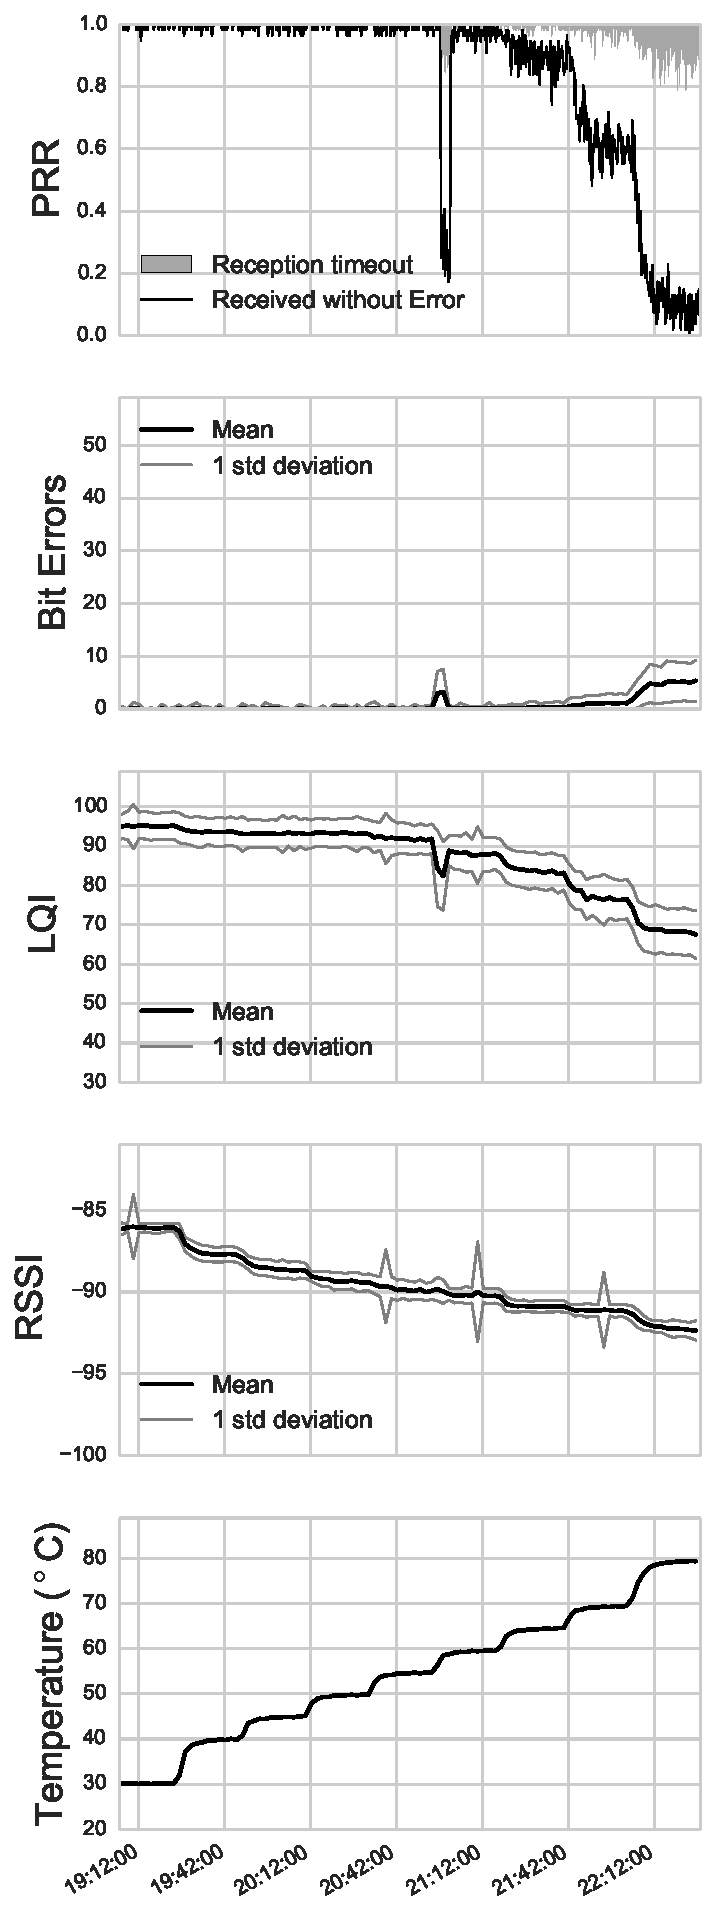
\includegraphics[width=0.475\columnwidth]{figures/prr_0-1_receiver}
		\label{fig:prr_link_01_receiver}
	}
	\caption{\acs{PRR} and link quality of messages received by mote \textbf{1} vs. temperature. For transmitter temperature see Figure~\ref{fig:prr_link_10}.}
	\label{fig:prr_link_01}
\end{figure}

\begin{figure}[t]
	\subfigure[Increasing receiver, constant \newline transmitter temperature.] {
		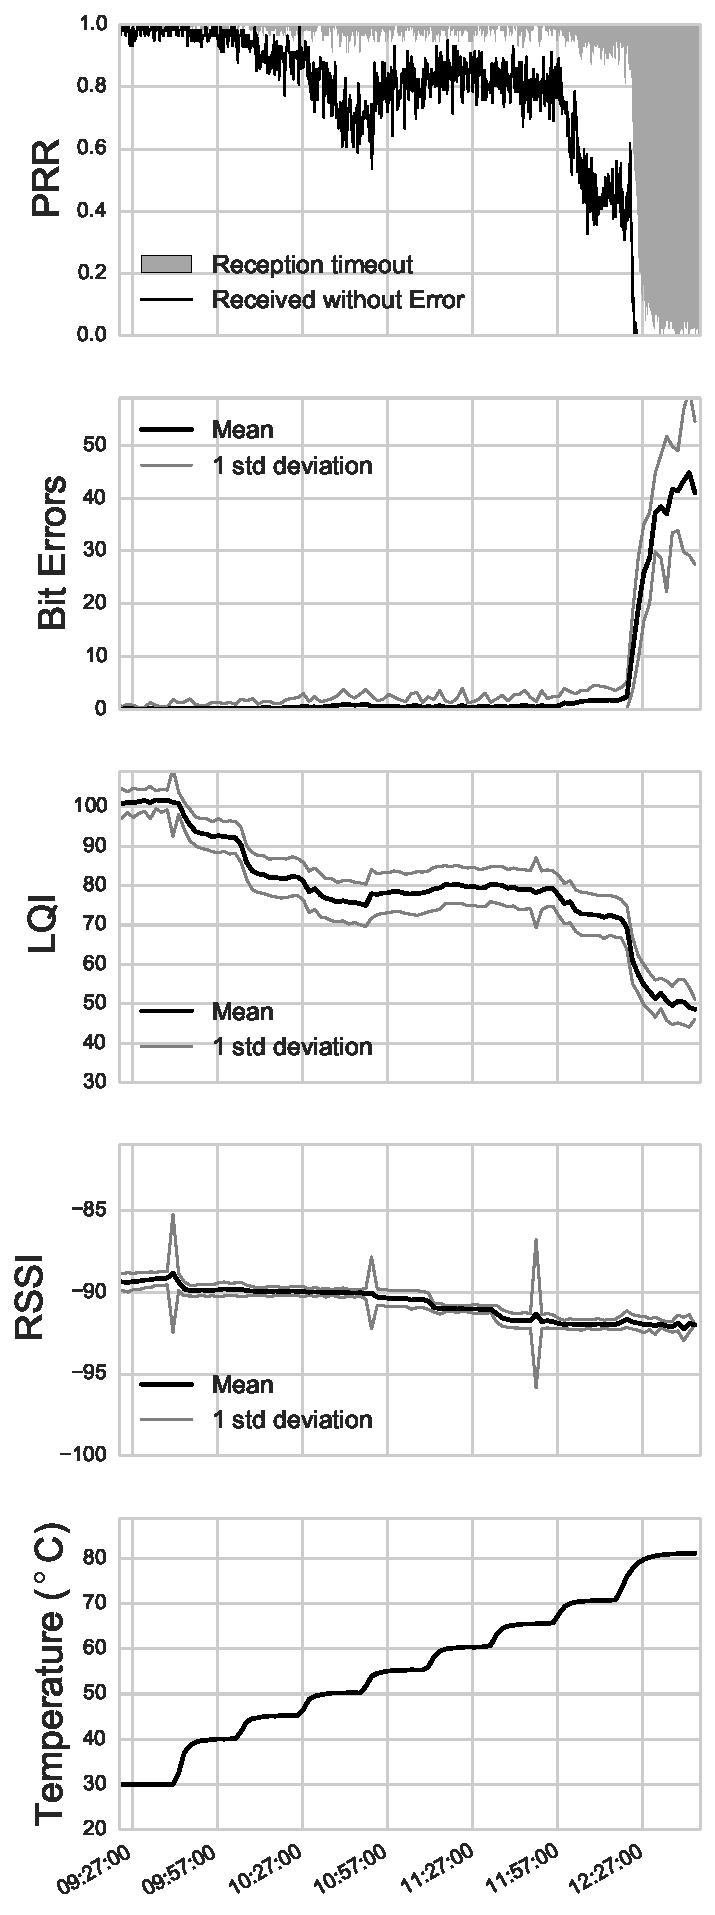
\includegraphics[width=0.475\columnwidth]{figures/prr_1-0_receiver}
		\label{fig:prr_link_10_receiver}
	}
	\subfigure[Constant receiver, increasing \newline transmitter temperature.] {
		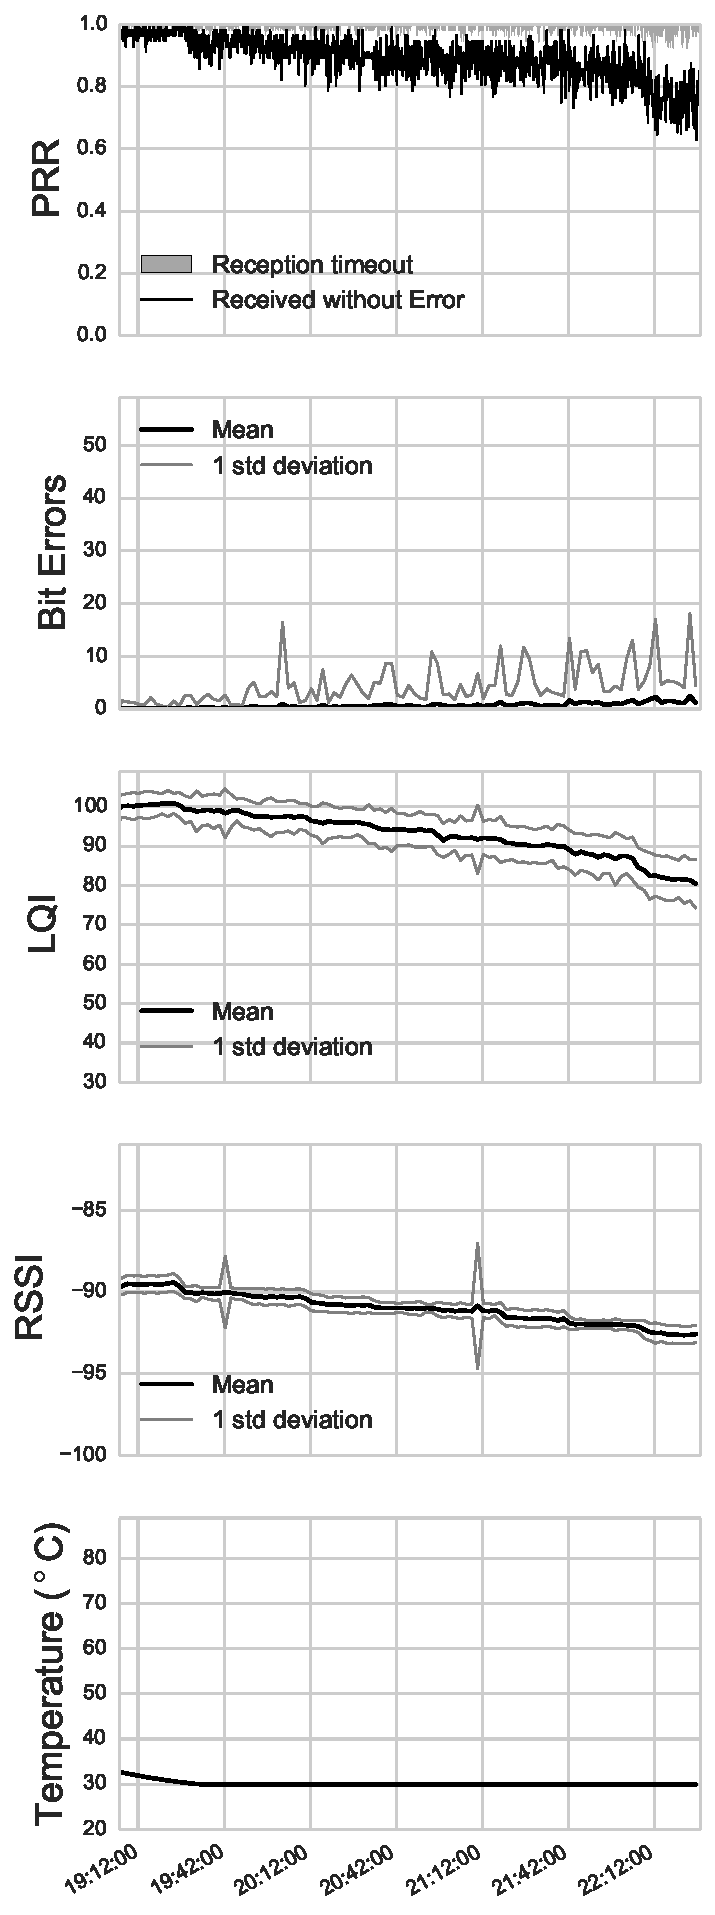
\includegraphics[width=0.475\columnwidth]{figures/prr_1-0_transmitter}
		\label{fig:prr_link_10_transmitter}
	}
	\caption{\acs{PRR} and link quality of messages received by mote \textbf{0} vs. temperature.  For transmitter temperature see Figure~\ref{fig:prr_link_01}. The asymmetry in \acs{PRR} shows much more cleary here.}
	\label{fig:prr_link_10}
\end{figure}

\subsection{Discussion}

These results are not necessarily incompatible with the findings of Boano~\etal{}, since the authors only looked at an effective temperature range of $0 - 65\,^{\circ}\mathrm{C}$, which is exactly the range, where we see little asymmetry in our experiment.
It is therefore feasible that there are link configurations in this temperature range, where this behavior can manifest itself.
However, our data strongly implicates the receiver as being more vulnerable than the transmitter to an increase in temperature, especially above $65\,^{\circ}\mathrm{C}$.

This link asymmetry can lead to some interesting situations, where a mote at high temperature is able to transmit messages, but not receive them.
Looking at their own temperature, mote would receive another hint in whether the lack of received messages is caused by a missing transmitter, or by its own disability to receive messages.
For example, when no messages are received after a timeout, a failure of the transmitter is more likely when the receiver is at low temperature than at high temperatures.

In a system that makes smart decisions based on information from multiple motes, such information could be used to judge whether the system is still functionally intact and then trigger a backup program, which reacts autonomously to the local sensor data collected but still notifies the rest of the network of its actions.
Motes that are not in this backup mode can very likely receive these transmissions and augment the group decisions with the constraints of these autonomously acting motes.
Therefore a failure of the entire system is delayed or prevented, by using controlled degradation of the system, which might not be as smart as before, but at least still providing a rudimentary service.

































